\chapter{Introduction}
\label{ch:intro}

"Lorem ipsum dolor sit amet, consectetur adipiscing elit, sed do eiusmod tempor incididunt ut labore et dolore magna aliqua. Ut enim ad minim veniam, quis nostrud exercitation ullamco laboris nisi ut aliquip ex ea commodo consequat. Duis aute irure dolor in reprehenderit in voluptate velit esse cillum dolore eu fugiat nulla pariatur. Excepteur sint occaecat cupidatat non proident, sunt in culpa qui officia deserunt mollit anim id est laborum."

Should probably mention somewhere that this is long-range PA, in contrast to short-range stuff being explored now.

\cite{Aman2018}

\section{Few-body physics}
\label{sec:few-body}

\section{Halo molecules}
\label{sec:halo}

\section{Properties of strontium}
\label{sec:sr}

\begin{figure}
\label{fig:energy_level_diagram}
	\centerline{
	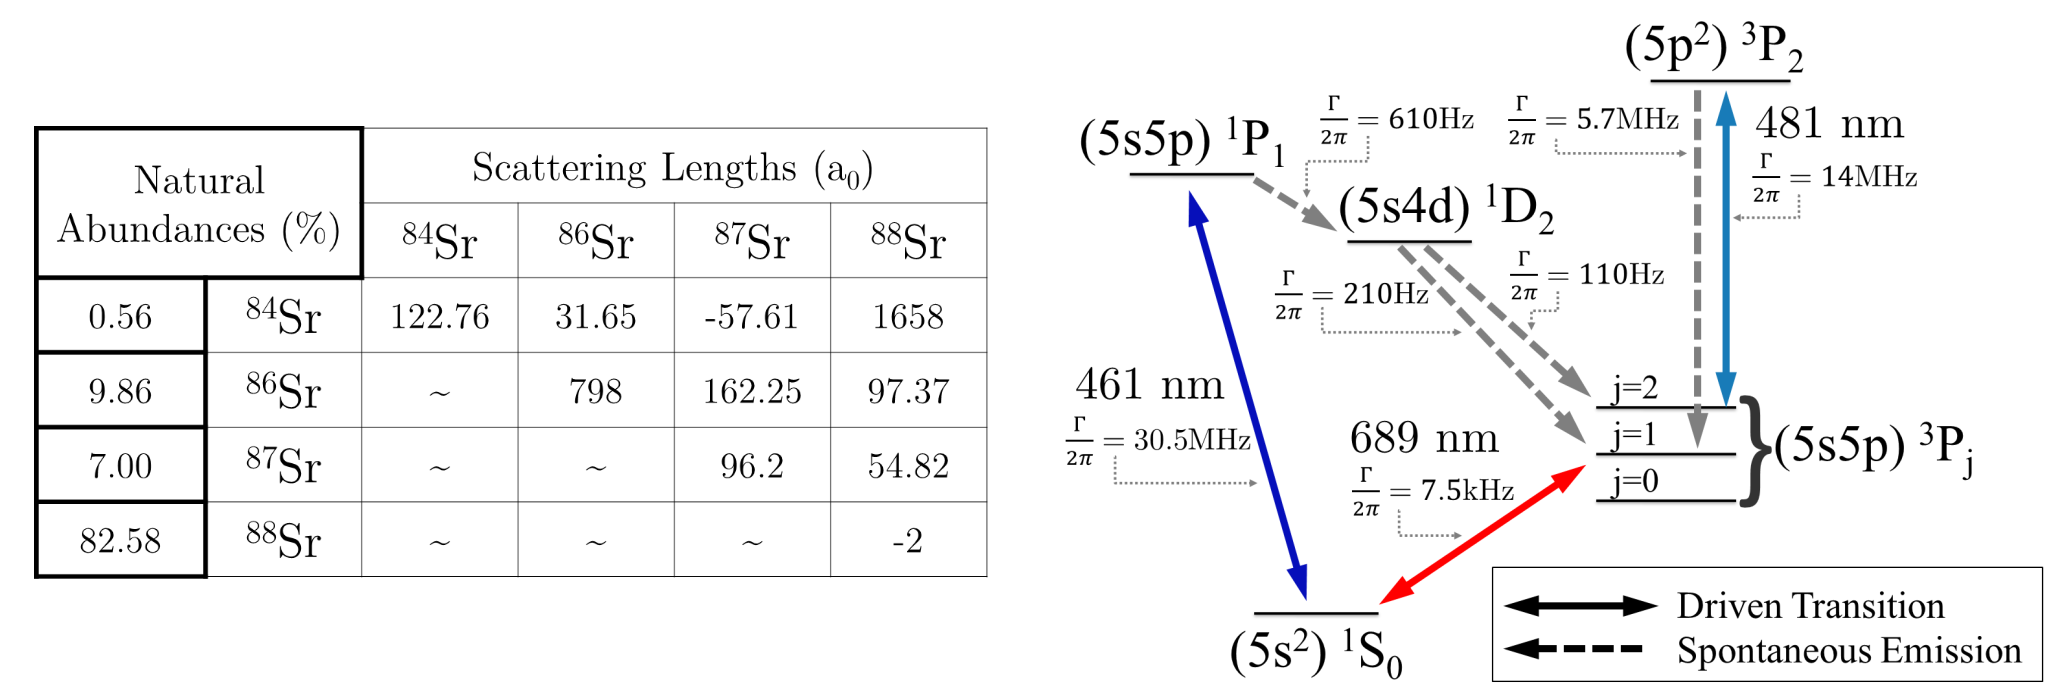
\includegraphics[height=0.25\textheight]{strontium_properties.pdf}}
	\caption{Properties of strontium}{Properties of strontium. Left: Natural abundances and s-wave scattering lengths for all mixtures of Sr. Right: Simplified energy level diagram of Sr showing the relevant states used for trapping and cooling of the atomic gas}
\end{figure} 

\section{Thesis Outline}
\label{sec:outline}


\begin{equation} 
\label{eq:1dlattice}
		 V(x) = V_{lat} \; \sin^2(k_L x)
\end{equation}



